\section{矢量数据库的原理}

本章节将介绍矢量数据库的原理,包括矢量索引编排、矢量查询和矢量后处理,从而详细介绍矢量数据库是如何工作的,揭开其神秘面纱。

\subsection{总览}

矢量数据库通过若干算法的组合实现了数据库功能,这些算法组合成一个管道进行运作。如图\ref{fig:pipe}所示,矢量进行索引编排后存入矢量数据库中,之后通过最近邻等方式进行查询,并进行后处理以得到最终结果。

\begin{figure}[H]
    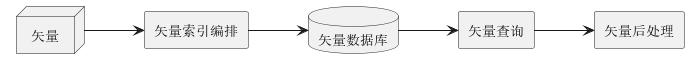
\includegraphics[width=\textwidth]{examples/pipe.png}
    \centering
    \caption{矢量数据库的算法管道}
    \label{fig:pipe}
\end{figure}

其中各个步骤的解释如下:
\begin{enumerate}
\item 索引编排。使用特定算法对矢量进行索引,将矢量映射到一个数据结构中,以实现更快的搜索。
\item 矢量查询。矢量数据库将索引的查询矢量与数据集中的索引矢量进行比较,以找到最近的邻居。
\item 矢量后处理。对最近邻矢量进行后处理以返回最终结果,这一步可以包括使用不同的相似性度量对最近的邻居进行重新排序。
\end{enumerate}

\subsection{矢量索引编排}

矢量索引编排用于将矢量映射到一个简化表示,并尽可能保留矢量中的信息,从而使得矢量可以在一个较低的维度进行快速比较。下面介绍几种索引编排算法。

随机投影\cite{bingham2001random}。随机投影的思想是通过一个随机数矩阵将矢量映射到目标维度,由于所有矢量通过相同的矩阵进行映射,只要矩阵设计合理,矢量就可以在低维空间中保持有效的关系。该算法可以表示为如下。

\begin{equation}
    V\times M\to V',
\end{equation}

其中$V\in\mathbb{R}^{K\times D}$表示原始矢量集合,$V'\in\mathbb{R}^{K\times D'}$表示映射后的矢量集合,$D,D'$表示映射前后的维度,$D\gg D'$。通过随机数矩阵$M\in\mathbb{R}^{D\times D'}$与原始矢量集合进行点乘,就可以得到映射后的矢量集合。

\begin{figure}[H]
    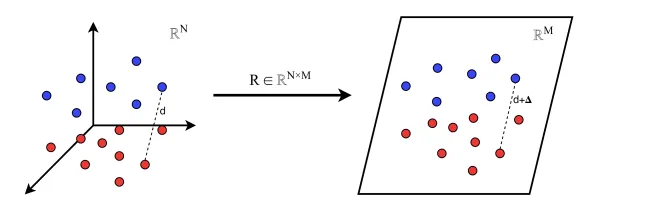
\includegraphics[width=\textwidth]{examples/random projection.png}
    \centering
    \caption{随机投影算法}
    \label{fig:rand_proj}
\end{figure}

图\ref{fig:rand_proj}展示了一个随机投影算法的示例,对于一个$N=3$维的立体数据集合而言,通过矩阵$R\in\mathbb{R}^{M\times N}$,就可以将数据映射到$M=2$维的平面数据集合。

乘积量化\cite{jegou2010product}。乘积量化是一种矢量有损压缩技术,通过将原始矢量分割为若干块,并为每个块生成代表性的代码来简化表示。其步骤如下:

\begin{enumerate}
    \item 矢量分割。将矢量分割为若干段。
    \item 代码生成。对每个段通过聚类算法得到若干簇,所有簇的聚类中心组成每个段的代码,每个代码拥有一个ID号。
    \item 矢量查询。将矢量转换为若干代码的表示后,通过代码的ID号集合找到最相近的矢量。
\end{enumerate}

该算法的准确率和性能视聚类中心数量而定。聚类中心越多,即聚类越细致时,该算法的查询越准确,然而速度也越慢;反之,虽然速度更快,查询却会更不准确。因此该算法需要根据实际情况进行合适的权衡。

\begin{figure}[H]
    \centering
    \subfloat[]{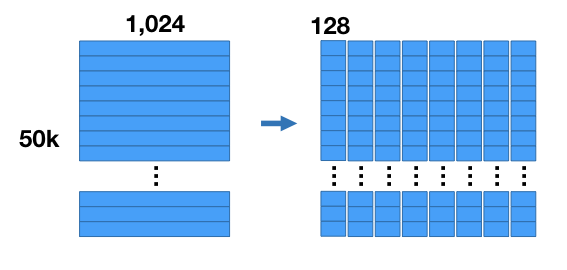
\includegraphics[width=0.5\textwidth]{examples/product quantization-step1.png}}
    \subfloat[]{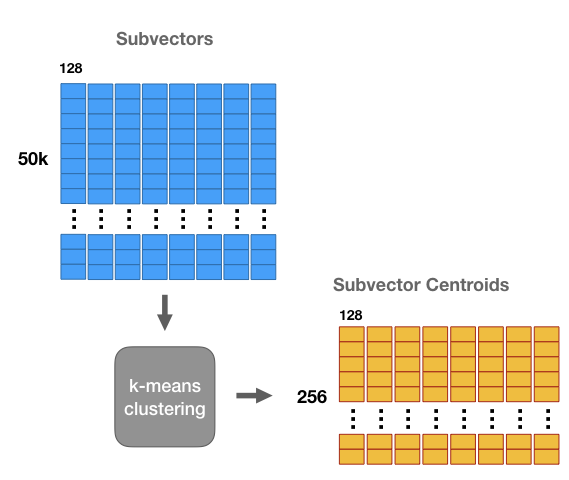
\includegraphics[width=0.5\textwidth]{examples/product quantization-step2.png}} \\
    \subfloat[]{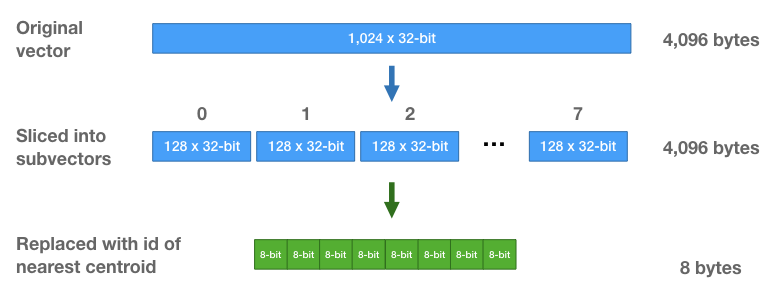
\includegraphics[width=1.0\textwidth]{examples/product quantization-step3.png}}
    \caption{乘积量化算法}
    \label{fig:prod_quan}
\end{figure}

图\ref{fig:prod_quan}展示了乘积量化算法的具体步骤。子图\(a\)表示矢量分割,1024维矢量被分割为8个128维的矢量段。子图\(b\)表示代码生成,通过KMeans聚类算法将每个段分为256个簇,并将簇中心的集合作为代码集合。子图\(c\)表示矢量查询,原始矢量通过分割和寻找最近邻代码之后得到一个低维表示,256个簇ID只需要8bit即可表示,而8个段总共只需要$8\times 8bit=64bit$,最后只需要在压缩后的表示空间中寻找最近邻即可。基于乘积量化算法,矢量被大大压缩了。

局部敏感哈希\cite{datar2004locality}。局部敏感哈希是一种近似最近邻的算法,对于一般的哈希函数来说,当内容发生微小变化后,哈希值就会发生无法预估的变化。而对于局部敏感哈希来说,内容发生微小变化后,内容也只发生微小变化甚至不变。于是,矢量在哈希空间中被映射到若干桶中,很容易找到最近邻。

一个简单的符合上述条件的哈希函数是:

\begin{equation}
    H(V)=|V\cdot R+b|/a,
    \label{eq:lsh1}
\end{equation}

公式\ref{eq:lsh1}展示了一个简单的局部敏感哈希函数,其中$R$是一个随机数矩阵,$b$是$[0,a]$之间均匀分布的随机变量,$a$是桶宽。当$R\in\mathbb{R}^{D\times 1}$时,所有矢量被映射到一条直线上,该直线被划分为若干长度为$a$的线段,每个向量会随机映射到不同的线段上。

还有一种局部敏感哈希函数是基于bit采样的哈希函数:

\begin{equation}
    H(V)=V[i],
    \label{eq:lsh2}
\end{equation}

公式\ref{eq:lsh2}中$V[i]$表示矢量$V$在第$i$位的值,将矢量二值化为元素0和1组成之后,就可以通过该函数在某个位上比较两者是否相同。

此外还有基于聚类、汉明距离等思想的局部敏感哈希函数,这里就不一一列举了。

\begin{figure}[H]
    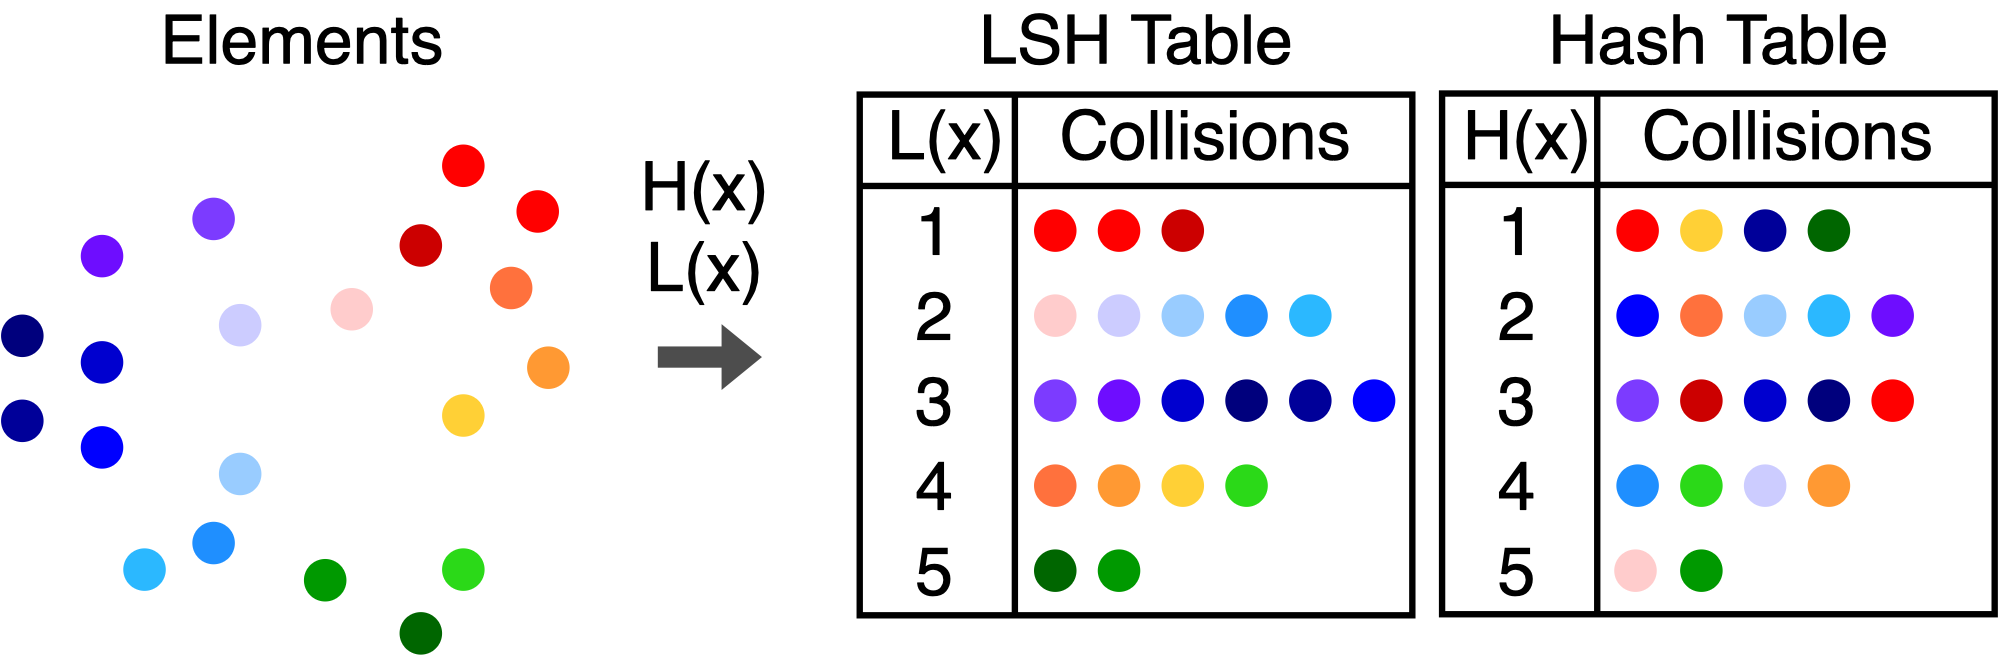
\includegraphics[width=\textwidth]{examples/lsh.png}
    \caption{局部敏感哈希算法}
    \label{fig:lsh}
\end{figure}

图\ref{fig:lsh}展示了局部敏感哈希的思想。图中$H(x)$表示普通的哈希函数,经过哈希后,不同哈希值对应的矢量集合很难有规律可循。而$L(x)$表示局部敏感哈希函数,经过哈希后,相似的矢量集合被分配到一起。

\subsection{矢量查询}

矢量查询基于对编排后的索引计算相似度来找到最近邻,一些常见的相似度度量方式有:

\begin{itemize}
    \item 余弦相似度。测量矢量空间中两个矢量之间的角度的余弦值。它的范围是$-1$到$1$,其中$1$代表矢量方向完全相同,$0$代表矢量方向正交,$-1$代表矢量方向完全相反。
    \begin{equation}
        \cos(V^1,V^2)=\frac{V^1\cdot V^2}{\Vert V^1\Vert\Vert V_2\Vert}=\frac{\sum_{i=1}^Nv_i^1v_i^2}{\sqrt{\sum_{i=1}^N(v_i^1)^2}\cdot\sqrt{\sum_{i=1}^N(v_i^2)^2}},
        \label{eq:cos}
    \end{equation}
    公式\ref{eq:cos}表示了余弦相似度的计算,其中$V^1,V^2$代表两个长度为$N$的矢量,$v_i^j$表示第$j$个矢量的第$i$个元素。
    \item 欧氏距离。测量矢量空间中两个矢量之间的直线距离。它的范围从$0$到无穷大,其中$0$代表矢量完全相同,较大的数值代表矢量越不相似。公式见\ref{eq:knn}。
\end{itemize}

\subsection{矢量后处理}

矢量后处理即根据用户需求来过滤需要的结果,用户的需求通常以元数据的形式表示。元数据可能是矢量的一些描述性信息,对于图像数据来说,元数据可能是照片拍摄时间、地点;对于文本数据来说,元数据则可能是文档来源、作者信息等。总之元数据是由用户需求指定的一些描述性的辅助信息。

为了实现基于元数据的过滤,在维护一组矢量索引以外,矢量数据库还需要维护一组元数据索引,并根据元数据执行过滤。矢量数据库的过滤方法在步骤上可以分为两种:预过滤和后过滤。

\begin{figure}[H]
    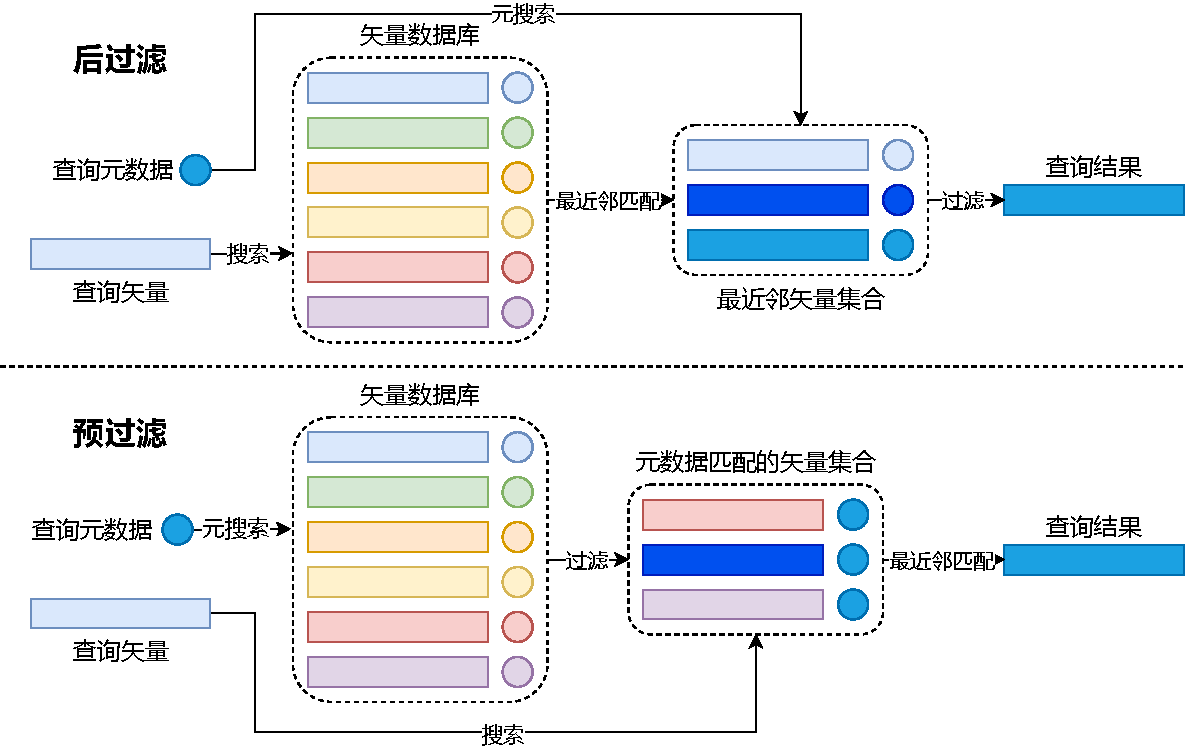
\includegraphics[width=\textwidth]{examples/filter.pdf}
    \centering
    \caption{矢量后处理流程}
    \label{fig:filter}
\end{figure}

图\ref{fig:filter}展示了矢量的后处理流程,其方法有两种:

\begin{itemize}
    \item 预过滤。元数据过滤在矢量搜索之前进行。虽然这有助于减少搜索空间,但它也可能导致系统忽略那些不符合元数据过滤标准的相关结果。
    \item 后过滤。元数据过滤在矢量搜索之后进行。这有助于确保所有相关的结果都被考虑在内,但它也可能引入额外的开销并减慢查询过程,因为不相关的结果需要在搜索完成后被过滤掉。
\end{itemize}

预过滤和后过滤策略都有各自的优缺点,需要视实际情况而定。